% Copyright [2018] E-train-Liu

%Licensed under the Apache License, Version 2.0 (the "License");
%you may not use this file except in compliance with the License.
%You may obtain a copy of the License at

%    http://www.apache.org/licenses/LICENSE-2.0

%Unless required by applicable law or agreed to in writing, software distributed under the License is distributed on an "AS IS" BASIS,
%WITHOUT WARRANTIES OR CONDITIONS OF ANY KIND, either express or implied.
%See the License for the specific language governing permissions and limitations under the License.
%%%%%%%%%%%%%%%%%%%%%%%%%%%%%%%%%%%%%%%%%%%%%%%%%%%%%%


\documentclass[12pt]{article}
\usepackage{xeCJK}
\usepackage{fontspec}
\usepackage{setspace}
\usepackage{listings}
\usepackage{color}
\usepackage{graphicx}
\usepackage{geometry}

\geometry{left=2.2cm, right=2.2cm, top=2cm, bottom=2cm}
\definecolor{vscode_normal}{rgb}{0.98,0.98,0.98}
\definecolor{vscode_background}{rgb}{0.16,0.16,0.16}
\definecolor{vscode_darkgreen}{rgb}{0.43,0.67,0,27}
\definecolor{vscode_blue}{rgb}{0.35,0.61,0.84}
\definecolor{vscode_darkyellow}{rgb}{0.93,0.49,0.19}
\definecolor{vscode_ruler}{rgb}{0.3,0.3,0.3}

\lstset
{
    basicstyle=\normalsize\ttfamily\color{vscode_normal},
    numbers=left,
    numberstyle=\normalsize\ttfamily\color{black},
    tabsize=4,
    breaklines=true,
    backgroundcolor=\color{vscode_background},
    commentstyle=\color{vscode_darkgreen},  
    keywordstyle=\color{vscode_blue},
    stringstyle=\color{vscode_darkyellow},
    showstringspaces=false
}

\setCJKmainfont[BoldFont=Noto Sans CJK SC Bold]{Noto Sans CJK SC Regular}
\setCJKmonofont{黑体}
\setmainfont{Open Sans}
\setmonofont{Ubuntu Mono}

\title{Octave Vol.1——新手高效Debug建议}
\author{E-train Liu}
\date{2018-05-05}

\begin{document}
\begin{spacing}{1.4}

\tableofcontents


\maketitle
\begin{center}
\large{关键词:高效debug,Octave,新手}
\end{center}


\includegraphics[width=\linewidth]{titlePicture.png}

“夜不美,代码太危险,总有人黑着眼眶熬着夜”。哦,不对,应该是“总有‘猿’黑着眼眶熬着夜”,程序猿。

上个周末到现在,我的微信里几乎让我帮着debug的。很显然,目前对于大多数人,除了没有思路,写出的代码跑不过也是相当大的一个问题。实际上,debug困难,一是因为开发经验不足,容易掉坑;二是因为没有良好的debug技巧,掉进坑里扑棱半天爬不出来。对于第一个问题,解决方法当然是多进行一些编程积累经验,这个肯定需要时间,coursework的DDL就在眼前了,这招估计赶不及。显然,第二种方法对于大部分人来说,是在短时间内快速提升的方法。

这篇很早就开始写了,零零碎碎写了好几篇,本来想暑假发。但是现在大家拔光了头发也找不到bug的情形让我想起我刚入坑时“编程5分钟,纠错两小时”的惨痛经历。感同身受之余,草草把这个合成一篇放了出来,希望解大家CW的燃眉之急。文章比较长,大家可以先看目录,再决定看哪一部分。如果发现有问题,欢迎在Issue中报给我,感谢不尽。

\section{三大类Bug}

虽然程序写的不怎也样,说说行业内部的黑话装个逼还是很必要的。Bug这个词的发明人是计算机上古时期的大佬Grace Hopper和她的团队,他们的计算机电路有一次被飞进去的虫子弄坏了,于是他们就用bug表示计算机错误,debug表示找错。

正如能弄坏电脑的虫子有很多种,能搞乱程序的bug也是有分类的。知道bug的种类有助于debug。

第一种叫做语法错误,就是写出了不符合语法规范的代码,导致计算机不认识了。比如说写错变量名、函数名,少写了”\texttt{endif},还有令“生灵有倒悬之危”的赋值语句\texttt{1 = a}等等。

第二种叫语义错误。简而言之就是逻辑有问题的程序。比如要求把\texttt{a}和\texttt{b}两个变量的和赋给\texttt{c},但是代码写成了\texttt{c = a * b},这类程序往往计算机能正常运行,但是运行结果不对。

第三种叫做运行错误。这类问题的原因一般是傻逼用户和穷逼系统。如果你写了一个递归法算一个数的迭乘的程序,有人却往里面输了一个字符,或者递归太多系统内存不够了,都属于运行错误。

\section{解决语法错误:善用错误和警告}

\subsection{错误和警告}

如果解释器报告错误(error),说明程序中有一个bug,这个bug严重到导致程序不能继续运行。如果发出的是“警告”,说明解释器发现了并不影响运行,但可能有错误的代码。或者是说这样的代码有造成问题的可能。

\subsection{善于利用错误和警告}

有些人程序一出错,立刻就要去抱大佬的们的大腿。然后各种承诺,请星巴克,求情,卖萌,递女装,自己女装/男装……咳咳,各种方法都用了。然而解释器早已经看透了一切,并且给出了高质量的错误说明。不会看解释器的报错是会严重拉低编程效率的。

例如编写下面这样一个程序

\begin{lstlisting}[language=octave]
function result = isEven1(number)
    % There is an error in this function.
    if mod(number, 2) === 0
        result = true;
    else
        result = false;
    endif
endfunction
\end{lstlisting}

运行结果如下:

\begin{lstlisting}
>> isEven(4)
parse error near line 3 of file /home/user/octaveFiles/isEven1.m

  syntax error

>>>     if mod(number, 2) === 0
                            ^
\end{lstlisting}

第一行是输入的命令,不用管。注意看第二行里有“near line 3”的字样,说明错误出在第三行上。倒数第二行是报错的代码,在最下面一行,还用“$\wedge$”标出了错误的位置。这个报错还是相当贴心而准确的。

还是相似的代码,当然还是有错误的

\begin{lstlisting}[language=octave]
function result = isEven2(number)
    % There is an error in this function.
    if mod(number, 2) = 0
        result = true;
    else
        result = false;
    endif
endfunction
\end{lstlisting}

运行结果如下

\begin{lstlisting}
>> isEven2(4)
warning: suggest parenthesis around assignment used as truth value near line 3, column 23 in file '/home/user/octaveFiles/isEven2.m'
ans = 0
\end{lstlisting}


\includegraphics{nottingduck_qurstionmark.png}

WTF?如果你直接看下面的\texttt{ans}的话,会发现运行结果是0(\texttt{false}),难道4不是偶数吗?显然现在程序能运行,但是有bug。来看一下上面的warning:

\begin{lstlisting}
2: warning: suggest parenthesis around assignment used as truth value near line 3, column 23
\end{lstlisting}

意思是说,建议在3行23列处插入能作为“true”的语句,这说明那个原来的语句的值永远为“false”。那么我们滚去源代码的第3行看一下

\begin{lstlisting} [language=octave]
3:         if mod(number, 2) = 0
\end{lstlisting}

看出问题来了吗?也许你不能明白这个语句的值为什么永远是“\texttt{false}”,但你应该能发现,这里赋值符号“=”被误用作了判断相等的“==”。可见,虽然警告不影响运行,但并不代表程序没有错。而这里,利用警告,我们成功找到了错误的点。

那为什么这个语句永远是“\texttt{false}”?这里要提到一个补充知识点,赋值语句也是有返回值的。只要赋值成功,那么就会返回等号右边的值。我们可以用下面的代码直接在octave的终端里验证一下:

\begin{lstlisting}
>>printf("%i\n", (a = 5));
\end{lstlisting}

输出结果是

\begin{lstlisting}
5
>>
\end{lstlisting}

这说明\texttt{(a = 5)}这整个式子的值是5。验证了我们刚才的说法

至此,我们可以积累一个经验,\textbf{一旦程序报出要“插入真值或假值”那样的警告,我们就应该考虑是不是混用了“=”和“==”。}

\subsection{报错位置不一定准确}

刚才说过,报错时会显示行号甚至是位置,但这不一定是好事。有时候会帮助我们找到错误,但有时候会误导我们。

例如下面这个程序

\begin{lstlisting}[language=octave]
function printNumbers(number)
% There is an error in this program.
    for i = 1 : number
        disp(i);
    for j = number : -1 : 1
        disp(j);
    endfor
endfunction
\end{lstlisting}

简单说一下,这个程序就是从\texttt{1}打印到\texttt{number},再从\texttt{number}打印到\texttt{1}。运行结果如下:

\begin{lstlisting}
>> printNumbers(12)
parse error near line 7 of file /home/user/octaveFiles/printNumbers.m
    
'for' command matched by 'endfunction'
    
>>> endfunction
    ^
\end{lstlisting}


\includegraphics{throwDesk.png}

坑爹啊,“\texttt{'for' command matched by 'endfunction'}”?电脑你有病吧,乱划鸳鸯谱把这两个配一对干什么啊!

然后再看报错,说问题出在第7行第1个字符上,去看一下

\begin{lstlisting}
7: endfunction
\end{lstlisting}

然而检查了\textit{n}遍后,发现这句并没有拼写错误什么的。其实这时,如果你死板的盯着报错里报的第7句看的话,即使过了DDL你也不会看出任何问题的。但是如果你浏览整篇代码,你倒是有可能发现,第3行的\texttt{for}缺少了对应的\texttt{endfor},即第4和第5行间应该加一个\texttt{endfor}。

那为什么不直接在第4行报错呢?我们来模拟一下Octave解释器逐行读取命令(“>>”的位置是读取的位置)。

\begin{lstlisting}[language=octave]
>>  function printNumbers(number)
    % There is an error in this program.
        for i = 1 : number
            disp(i);
        for j = number : -1 : 1
            disp(j);
        endfor
    endfunction
\end{lstlisting}

第一步,如上面的代码,解释器先读到了一个\texttt{function}。

\begin{lstlisting}[language=octave]
    function printNumbers(number)
    % There is an error in this program.
>>      for i = 1 : number
            disp(i);
        for j = number : -1 : 1
            disp(j);
        endfor
    endfunction
\end{lstlisting}

接着,解释器读到了第1个\texttt{for}。

\begin{lstlisting}[language=octave]
    function printNumbers(number)
    % There is an error in this program.
        for i = 1 : number
            disp(i);
>>      for j = number : -1 : 1
            disp(j);
        endfor
    endfunction
\end{lstlisting}

此时,程序读到了第2个\texttt{for}。由于我们漏写了\texttt{endfor},程序没有读到\texttt{endfor}就会认为第1个\texttt{for}没有结束,而第2个for是嵌套在第1个for里的。

\begin{lstlisting}[language=octave]
    function printNumbers(number)
    % There is an error in this program.
        for i = 1 : number
            disp(i);
        for j = number : -1 : 1
            disp(j);
>>      endfor
    endfunction
\end{lstlisting}

程序读到了一个\texttt{endfor},所以解释器知道第2个\texttt{for}循环的代码至此结束。

\begin{lstlisting}[language=octave]
    function printNumbers(number)
    % There is an error in this program.
        for i = 1 : number
            disp(i);
        for j = number : -1 : 1
            disp(j);
        endfor
>>  endfunction
\end{lstlisting}

程序读到了\texttt{endfunction}。应该来说,这时候程序应该知道\texttt{function}结束了。但是Octave比较特殊,当一个\texttt{*.m}文件中只有一个\texttt{function}时,对于Octave来说有没有\texttt{endfunction}都差不多(但我并不建议不写\texttt{endfunction}!)。这时程序认为相比于缺少一个\texttt{function}的结尾,缺少一个\texttt{for}的结尾更要命,因此认为代码的问题是把与第一个\texttt{for}的结尾\texttt{endfor}写成了\texttt{endfunction}。于是出现了刚才画风清奇的报错结果。

By the way,有些版本的Octave对于上面那个程序的报错是“\texttt{'endfor' command matched by 'endfunction'}”。我不是特别明白其中的原理,为什么要把两个\texttt{end}配对,再次不敢妄言。可能是现在社会开放了,连编译器的取向都多样化了 [手动滑稽]。Anyway,如果有大佬知道其中原理的话,欢迎在Issue中分享一下。

至此我们又可以涨一个经验:\textbf{当程序对某行报错,但该行没有问题时,说明可能是代码中出现了匹配错误。我们此时就不应该仅拘泥于报错的行数,而应该浏览整篇代码中需要匹配\texttt{end}的语句。}

这样的经验十分重要。这能让我们更快的找一些坑爹指数高的bug。

例如下面一个猜数字的游戏。

\begin{lstlisting}[language=octave]
function guessNumber1()
% 一个让用户猜0-10整数的游戏
% 程序中有错误
    answer = round(10 * rand());
    %随机生成一个0-10的整数
    guess = input("Please input an integer in [0,10]: ");
    while guess != answer
        % 获取用户输入的猜测
        if guess < answer
            disp("Too small! Try again.");
        else if guess > answer
            disp("Too large! Try again.");
        endif
        guess = input("Please input another integer in [0,10]: ");
        % 重新再获取一次用户的输入
    endwhile
    disp("Congratulations! Your guess is correct!");
endfunction
\end{lstlisting}

这个程序运行结果如下

\begin{lstlisting}
parse error near line 16 of file /home/user/octaveFiles/guessNumber1.m

    'endif' command matched by 'endwhile'
  
>>> endwhile
    ^
\end{lstlisting}

一个没有任何经验的人如果看到这样的结果,第二天可能就有黑眼圈了。但是历史惊人的相似,报错行号不对,且又出现了乱配对的情况。我们已经有了上面的经验,可以直接推断,程序中出现了匹配错误。这样,我们就只看程序中需要“\texttt{end}”的语句就行了。

其中,\texttt{function},\texttt{while}和\texttt{if}语句都需要\texttt{if}。\texttt{function}和\texttt{while}比较简单,仔细检查一下就发现没错。那么下一步就需要好好抠一下这个\texttt{if}语句了。

\begin{lstlisting}[language=octave]
if guess < answer                   % Line 9
    disp("Too small! Try again.");  % Line 10
else if guess > answer              % Line 11
    disp("Too large! Try again.");  % Line 12
endif                               % Line 13
\end{lstlisting}

老实说,这个bug确实有点难了。对于这样的bug,一个土方法是根据解释器的报错猜测性的稍微改动一个地方,发现不行的话,再找另一个地方改。虽然这个方法可能很多人不用教都会,但在毫无头绪是也确实管事。当然,当我们对一个地方的错误总看不出来时,可以思考一下是不是我们本身的认知就有问题呢?带着死马当活马医的心态,我们看一下官方\texttt{help}中对\texttt{if}和\texttt{else}的解释。

\begin{lstlisting}
>> help if

-- if (COND) ... endif
-- if (COND) ... else ... endif
-- if (COND) ... elseif (COND) ... endif
-- if (COND) ... elseif (COND) ... else ... endif
    Begin an if block.

         x = 1;
         if (x == 1)
           disp ("one");
         elseif (x == 2)
           disp ("two");
         else
           disp ("not one or two");
         endif
...
\end{lstlisting}

发现官方例子中的\texttt{elseif}和我们的的不同之处了吗?官方的是“\texttt{elseif}”,两个单词连写,中间没有任何间隔。而我们的是“\texttt{else if}”,中间加了一个空格。

原来如此!“\texttt{elseif}”本身就是一个完整的命令,它是一个“\texttt{if}”语句的一部分。它应该长这样

\begin{lstlisting}[language=octave]
if condition1
    statement1
elseif condition2
    statement2
else
    statement3
endif
\end{lstlisting}

当我们加了空格之后,就相当于把它拆成了一个“\texttt{else}”和一个“\texttt{if}”。而拆出的\texttt{if}此时相当于被包含在\texttt{else}中,它本身是一个独立的\texttt{if},还需要一个\texttt{endif}。就像下面这熊样

\begin{lstlisting}[language=octave]
if condition1
    statement1
else  if condition2
        statement2
      else 
        statement3
      endif
endif
\end{lstlisting}

当然,这样写是不符合代码规范的,小朋友们千万不要学哦,会被其他读代码的人打的哦。正常情况下应该写成下面这样:

\begin{lstlisting}[language=octave]
if condition1
    statement1
else
    if condition2
        statement2
    else 
        statement3
    endif
endif
\end{lstlisting}

另外,那个猜数字的程序里获取用户输入的语句出现了两次,实际是写麻烦了。“\texttt{do...until}”语句了解一下。

\section{语义错误:试试断点法和输出变量法}

出现了语义错误的的话,很可能不报错不警告,这时候解释器的报错机制就救不了你了。

的确,这样的错误最好的方法就是自己认真的去重新阅读分析代码,显然这是个苦差事。但是,如果掌握了断点和输出变量的用法,那这个过程就会轻松很多。

\subsection{输出变量法}

输出变量调试法就是,在程序中加入一些语句,把程序变量的值打印出来。通过分析这些变量的变化,可以知道程序的问题所在。

当然,你可以用\texttt{disp()}或\texttt{printf()}打印所要监视的变量。但是这并不是一个简单的办法。别忘了,Octave自带一个属性,就是不加分号就打印变量。我们只要把要监视的变量后面的分号去掉就好了。

\subsection{断点法是什么黑科技?}

断点就是指在程序中设置一个位置。每次程序运行到这个位置时,就会暂时停下来。同时,程序会显示此时程序中各个变量的值。通过分析这些值,程序猿就能清楚的知道程序运行是否正常或其问题所在。

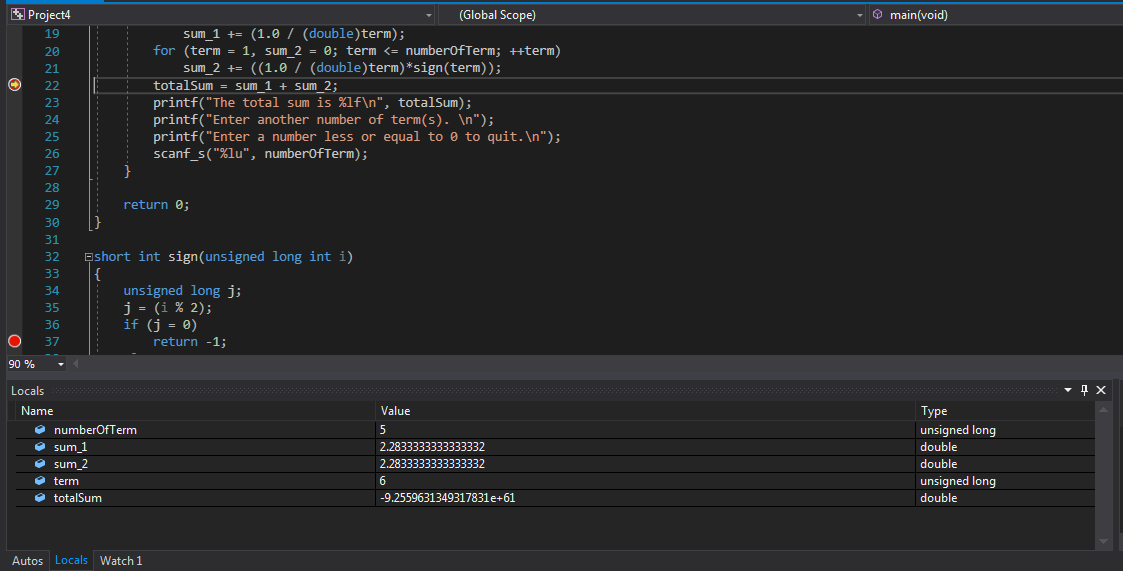
\includegraphics[width=\linewidth]{breakpoint_vs.png}

如图中用MS Visual Studio调试C语言,图中两个红点所在的那个行就是断点的位置,而有黄的箭头的那个断点是程序暂停的位置。而下方的窗格里有各个变量的类型和值。

其实说到这里,大家可能会发现,无论是输出变量法还是断点法,本质上都是使变量的值可视化。只不过,用变量输出法很可能会一下子打出来一坨,找到到底是第几步哪个位置出的毛病很折磨人,而让程序停下来看此时的变量,显然更方便。

\subsection{自己制造断点}

刚才所说的断点功能,主要是一些集成开发环境(IDE)和编辑器的插件提供的。(这两个词不认识不要怕,我应该会在下下次发文时进行解释)

“哇,这个‘断点’好厉害,Octave里在哪开啊?快说快说!”

很可惜,Octave貌似没有提供这样的黑科技。


\includegraphics[width=0.5\linewidth]{whatTheHell.png}

可能有人看到这里就有打我的冲动了:“没有你说它干嘛啊?增加我们心理落差?”诶诶,各位好汉别冲动,我们可是有创造世界能力的电子信息科技工程师俗称程序猿啊。原来没有的东西,按照程序员的创造探知精神,应该是自己动手丰衣足食,用奇淫巧技造出来啊!

首先,仔细想一下,断点法比输出变量法多的,就是能让程序暂停。那么我们只要用去分号的方法,就能实现显示变量的功能了。

好了,断点的第二个功能已经有了。至于第一个让程序停下来的功能么,实现方法就是,在我们想让程序停下的地方,暂时加上一个\texttt{input("");}。注意不用把这个\texttt{input();}的返回值赋给任何变量,但是必须给\texttt{input();}的括号里放一个字符串作为参数,否则这个函数就会因为缺乏参数而无法运行。如果想不到什么好的句子,就在括号里打个引号使其生成一个空字符串就行了。

这样做的原理就是,\texttt{input();}这个自带函数会让程序暂时停下来,然后等待用户输入一些东西。只有用户输入了什么并按下回车后,\texttt{input();}如愿以偿的拿到了它想要的输入,然后程序就会再次运行。如果你用这种方法暂停了程序,只需要随便输入点什么敲回车就能让程序重新跑起来。实际上,直接敲回车也是可以的,因为这样会输入一个回车符或者换行符。

这样,自制断点就大功告成了!


\includegraphics[width=0.5\linewidth]{thugLife.png}

\subsection{示例}

举一个例子来说明一下断点应该怎么用。下面是一个用于计算迭加的程序。

\begin{lstlisting}[language=octave]
function result = mySum(upperLim)
%程序有错误
    addedNum = 1;
    sum = 0;
    while addedNum < upperLim
        sum += addedNum;
        addedNum += 1;
    endwhile
    result = sum;
endfunction
\end{lstlisting}

该程序一个运行示例如下

\begin{lstlisting}
>> mySum(10)
ans = 45
\end{lstlisting}

但是,如果用公式自己算的话,从1加到10的结果应该是

\[ \rm{ 1 + 2 + \cdots + 10  = 10 \times \frac{1 + 10}{2} = 55 } \]

显然出错了。我们用自制断点法,去掉程序中的分号,然后在循环的最后加上一个\texttt{input},然后现在代码应该长这样

\begin{lstlisting}[language=octave]
function result = mySum(upperLim)
% 断点调试版本
    addedNum = 1
    sum = 0
    while addedNum < upperLim
        sum += addedNum
        addedNum += 1
        input("Paused. Press enter to continue."); % 断点在此
    endwhile
    result = sum
endfunction
\end{lstlisting}

现在建议再开一个窗口同样打开这份PDF,然后对照着刚才的代码看下面的分析。如果你的PDF阅读器不支持二开,网页浏览器可以一战。

重新再运行一次,等到第一次停下来时,屏幕上出现这样的内容

\begin{lstlisting}
>> mySum(10)
addedNum = 1
sum = 0
sum = 1
addedNum =  2
Paused. Press enter to continue.
\end{lstlisting}

运行结果中的第2、3行显然对应着源代码的3、4行。此时还没有进入循环。第4行又出现了一次\texttt{sum},这对应的是第6行,此时已经进入循环,并且第一次给\texttt{sum}加值了。当然从这里我们也可以看到,我们第一次给\texttt{sum}加了个\texttt{0}导致它的值没变,做了个无用功。这算不上是个bug,但也确实写得不怎么样。所以最好把\texttt{addedNum}的初始值设成1。

然后接下来就看着程序运行,每停一次,就看一下是不是正常,然后按回车再运行。

在第10和11次停的附近,我们会发现一些异常情况

\begin{lstlisting}
...
sum =  36
addedNum =  9
Paused. Press enter to continue.
sum =  45
addedNum =  10
Paused. Press enter to continue.
result =  45
ans =  45
\end{lstlisting}

可以看到,在上面第2行,\texttt{sum}是36,第3行时,\texttt{addedNum}已经递加为9,然后程序暂停了一下。接着到第5行,\texttt{sum}被加上了\texttt{addedNum}从而变成了45,\texttt{addedNum}也在第9行递加为10。现在,只要\texttt{sum}再加一个\texttt{addedNum},就得到正确答案了。

暂停后,却直接出现了\texttt{result}的值,说明已经退出了循环。显然此时已经不满足循环的判断条件了。看一下源代码中第5行,

\begin{lstlisting}[language=octave]
    while currentNum  < upperLim    % 第5行
\end{lstlisting}

\texttt{while}的判断条件是被加值小于最大值,而不能相等。这就是为什么到加不了最后的10。

也许有人会说这个错误太简单,没必要这样大费周章。其实这不过是一个例子而已。但是在思维受阻时,与其对着屏幕干瞪眼,不如用这种方法。还有,如果以后我们需要调试大型的复杂程序,断点会非常的高效。

\subsection{注意}

断点并非没有坏处,最明显的就是如果你交Coursework时,如果不把刚才去掉的分号补上,或者多加的\texttt{input}删去的话就凉了,你的Coursework会被扣掉相当可观的分数。在实际的开发中,调试完程序也必须把所有断点去除。

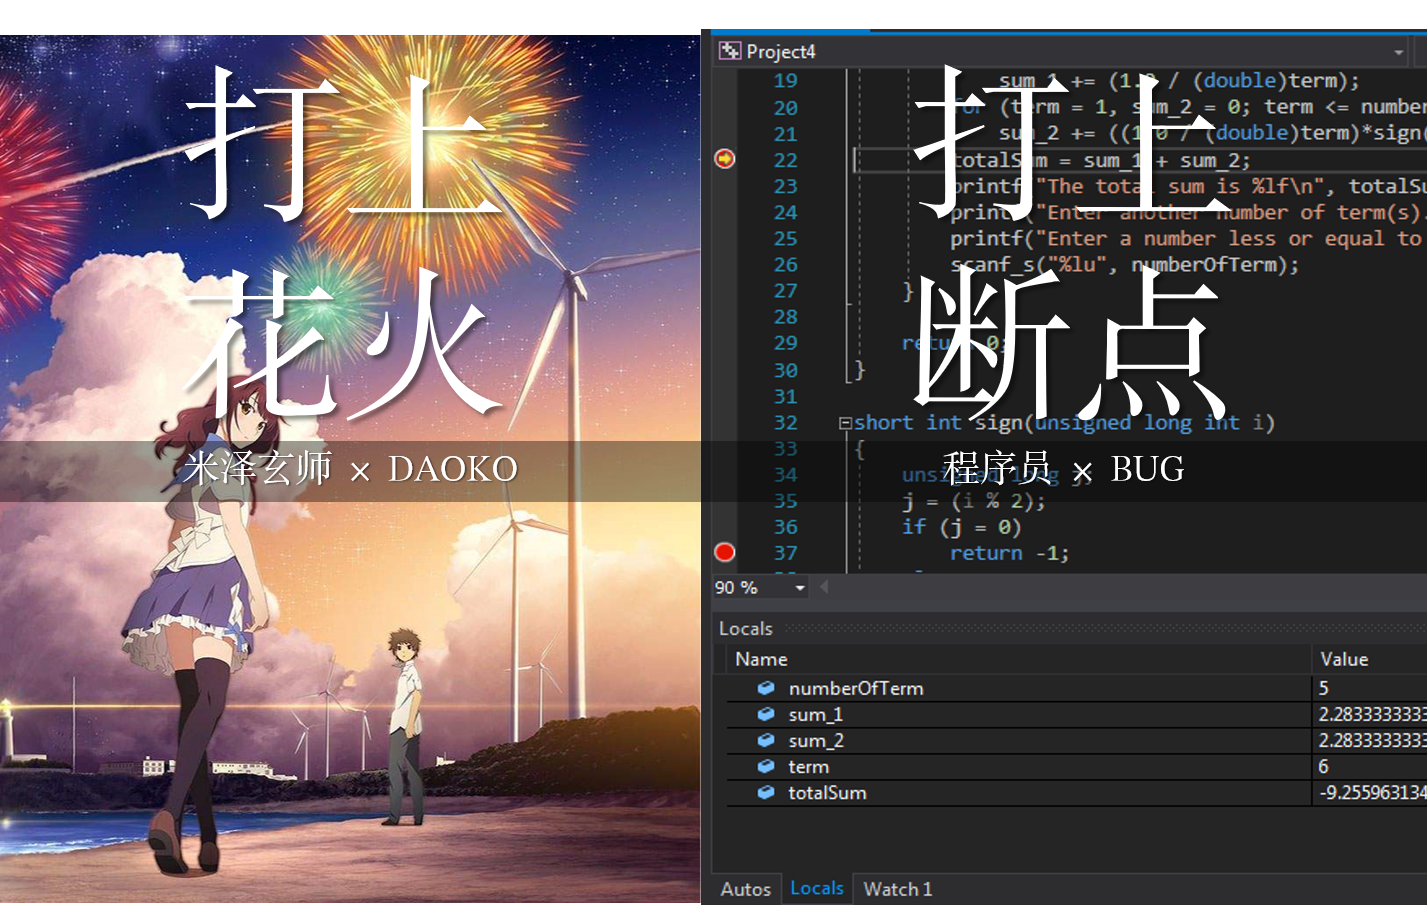
\includegraphics[width=\linewidth]{makeFirework&makeBreakPoint.png}

此外,断点也只是我们的辅助工具,不能代替我们自己对程序的分析思考。程序一出错,不分析代码,就打上一大堆断点的行为,实际上就是依赖电脑的帮助进行debug,放弃了对程序的思考。这样会使初学者的水平长期得不到提高。不说这些空话,就比如考试的时候写代码,如果没有自己纠错的能力,还能在试卷上打断点吗?

今天大课上,Manish(2018)有一句话说的很好,虽然记不得完全的原话,还是想分享给大家。

\textit{“The aim of this module, is to training your thought and logic, but not how to use functions. Because we want you to be a programmer, rather than just a user."}

\section{运行错误}

从上面对运行错误的原因的分析就能看出,运行错误没法像上面两个错误一样,那么容易被我们自己控制。关于防止用户瞎输入的方法的确有些复杂,也不是初学者应该过多关注度东西,我们大可到学C语言时再想它。

\subsection{递归导致的内存不足}

当然,比较常见而且能控制的一种运行错误,就是递归导致的内存不足。

比如Manish上课说过的一个阶乘函数,下面这个是递归版本

\begin{lstlisting}[language=octave]
function returnValue = fac_rec(num)
    if num == 1
        returnValue = 1;
    else
        returnValue = num * fac_rec(num - 1);
    endif
endfunction
\end{lstlisting}

下面这个是迭代版本
\begin{lstlisting}[language=octave]
function returnValue = fac_ite(num)
    returnValue = 1;
    for factor = 1 : num
        returnValue *= factor;
    endfor
endfunction
\end{lstlisting}

一些比较小的数字,两个函数,没有多大区别。当数字增大到100时,递归版本已经开始出现卡顿,而迭代版本依然秒开。当增大到300时,运行递归版出现了报错

\begin{lstlisting}
>> fac_rec(300)
error: max_recursion_depth exceeded
error: called from
    fac_rec at line 5 column 21
\end{lstlisting}

看第2行,这个 报错不是你的程序有错,而是达到了递归的最大深度,也就是递归太多内存不够了。而迭代版依然稳如老狗。虽然会出现“\texttt{ans = Inf}”表示结果过大,程序的当前的类型已经存不下了,因此被视为了无穷大(infinite)。当然,函数还是能跑而且很快的。

抱着挑战极限的心态试了一下,大约在\texttt{1.0e+6}(这是浮点数的科学计数法,也就是 $\textrm{1.0} \times \textrm{10} ^{\textrm{6}} $ )时出现了明显的卡顿和风扇的抗议声(指散热风扇,不是某大佬),\texttt{1.0e+10}时终于崩溃报错。

当然,不同机器上运行结果不一样,与处理器和内存都有关。Manish上大课时用学校电脑上的虚拟机试时,100左右递归版就GG了。

为什么递归和迭代的性能相差甚远?这个需要知道一点计算机底层的知识。当计算机运行过程中,会产生一些体积小但是需要快速访问的数据,他们会被存储在随机访问存储器(random access memory, RAM)也就是内存条中,而不是计算机的硬盘。一般来说个人计算机的RAM也就4-16 GB。而编程语言运行时,其中的一些数据会被存放到RAM中一个叫栈(stack)的区域。每一个函数运行时,相关的数据就会在栈中占据一定空间,行业黑话叫加了一个栈帧(stack frame)。而递归会多次调用函数,而且在被调用的函数返回值以前主调函数还不能返回值并停止,这样就导致大量的栈帧一层层的在栈中堆积,最终栈不够用了,程序就崩了。而迭代过程中,数据都只存放在几个变量中,每一次迭代这些变量值发生变化时,都会把上一次的数据覆盖而不会保留,因此迭代一般不会占用过多空间。

因此解决内存不够报错的方法,就是讲迭代改成等价的递归。这也是在实际的编程开发中迭代远比递归常用的一个原因。只熟悉递归而不熟悉迭代的同学,很抱歉,请忍痛割爱。

\subsection{系统差异引发的报错}

不知道你是否还记得,大明湖畔的Coursework 2的说明文档的Caution里,有这样一句话:

“\textit{If you create functions on your own computer it is your responsibility to ensure that they perform correctly on the UNNC system. You will lose marks for functions that will NOT run properly on UNNC computers; regardless of how they will perform on your own computer.}”

我们常用的操作系统是Windows和OS X,但上一届的有些学长提醒我们,学校用于验收作业的系统是Linux,所以要警惕在自己电脑上能跑但到学校电脑不能运行的情况。此外,不少Mac用户也反映,Octave在Mac上用户体验较差。其实Windows也不怎么样,因为目前UNNC学生的Windows都以Win10为主,然而Octave的安装软件和社区都有提示,实际上官方并没有正式做过Octave在Win10上的调试实验,现在的意见都是社区里的个人Win10用户提交的。Anyway,Octave本身就是Linux世界的产物,至于Os X和Windows,都是移植过去的,难免会有一些问题。所以还是建议在Linux的Octave上调试一下程序。

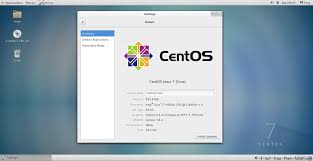
\includegraphics{centos.jpg}

Linux有非常多的发行版。目前个人用户中比较流行的是CentOS和Ubuntu。开始我比较推荐CentOS,因为以后如果有同学需要学习搭建Linux服务器的话CentOS比Ubuntu更稳定专业、更适合做服务器,而且和Manish是同款系统 [滑稽]。然而最近发现,CentOS官网上几个镜像下载下来的CentOS 7都是不自带图形化界面(GUI)的,对于新手来说自己装图形化界面有点麻烦。而且网上查到的个在CentOS上安装Octave方法,下载下来的Octave都是不带图型化界面的。所以,如果你和我一样是Linux小白,而且目前就是急着调试Octave的话,我推荐Ubuntu。而且刚才说Ubuntu不太专业也是和有一些Linux系统相比,和Win以及OS X相比当然还是更适合编程开发。如果有大佬知道怎么在CentOS下载有GUI的Octave的话麻烦分享一下。

至于怎么下载虚拟机和安装Linux,这里有一篇比较好的文章:https://blog.csdn.net/haoxiangtianxia/article/details/19993977。在此不再赘述了。但是这个教程中有一点我不太赞同,就是给Ubuntu分配1G的内存,亲测只有1G内存Ubuntu很容易卡死,建议至少1.5G,但也不要超过实际计算机内存的一半。还有,如果你是Windows用户,虚拟机默认会把虚拟盘放到C盘,那个虚拟盘能最大到10多个G,如果你的C盘不大,建议自己选择一个合适的路径放虚拟盘。另外,在去官网下载Ubuntu的光盘映像时,注意看一下你的机器是32位(x86)还是64位(x64),如果是32位那么你就不能装64位的系统。

安装好Ubuntu后,点击屏幕左下角,有点相当于安卓的“所有应用”。然后在里面找到终端(Teminal),点开。

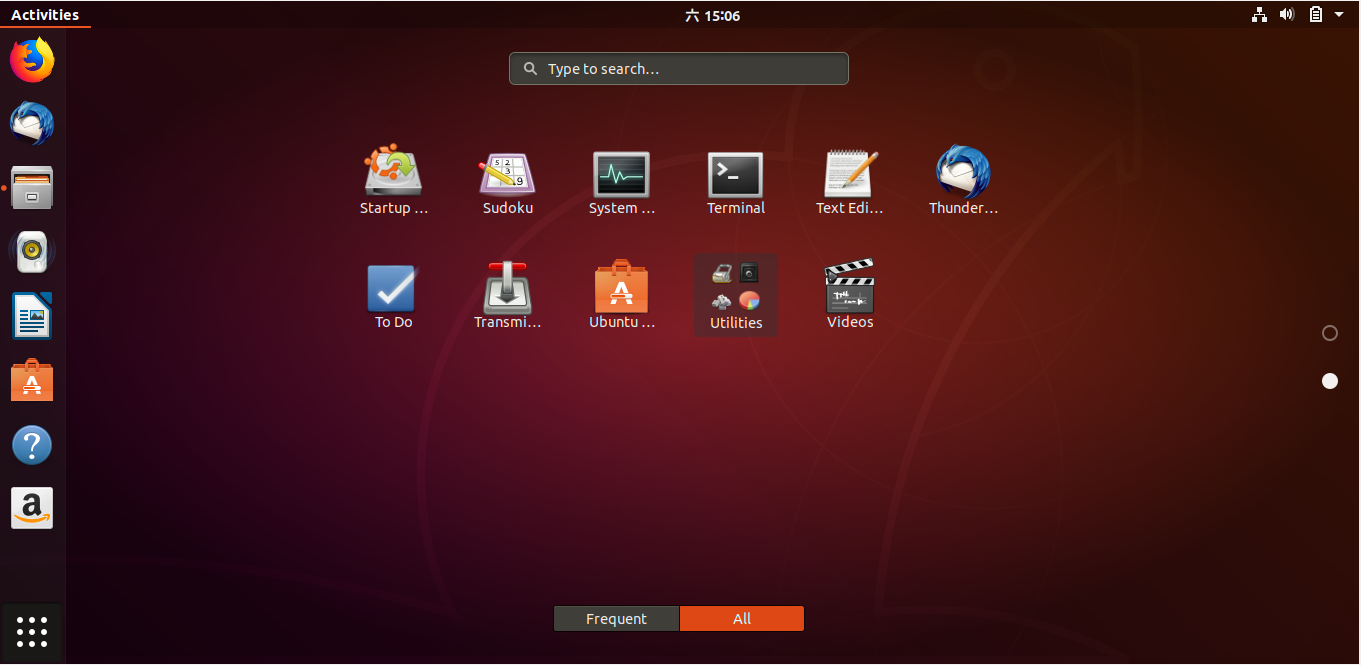
\includegraphics[width=\linewidth]{ubuntu1.png}

在里面输入

\begin{lstlisting}
sudo apt install octave    
\end{lstlisting}

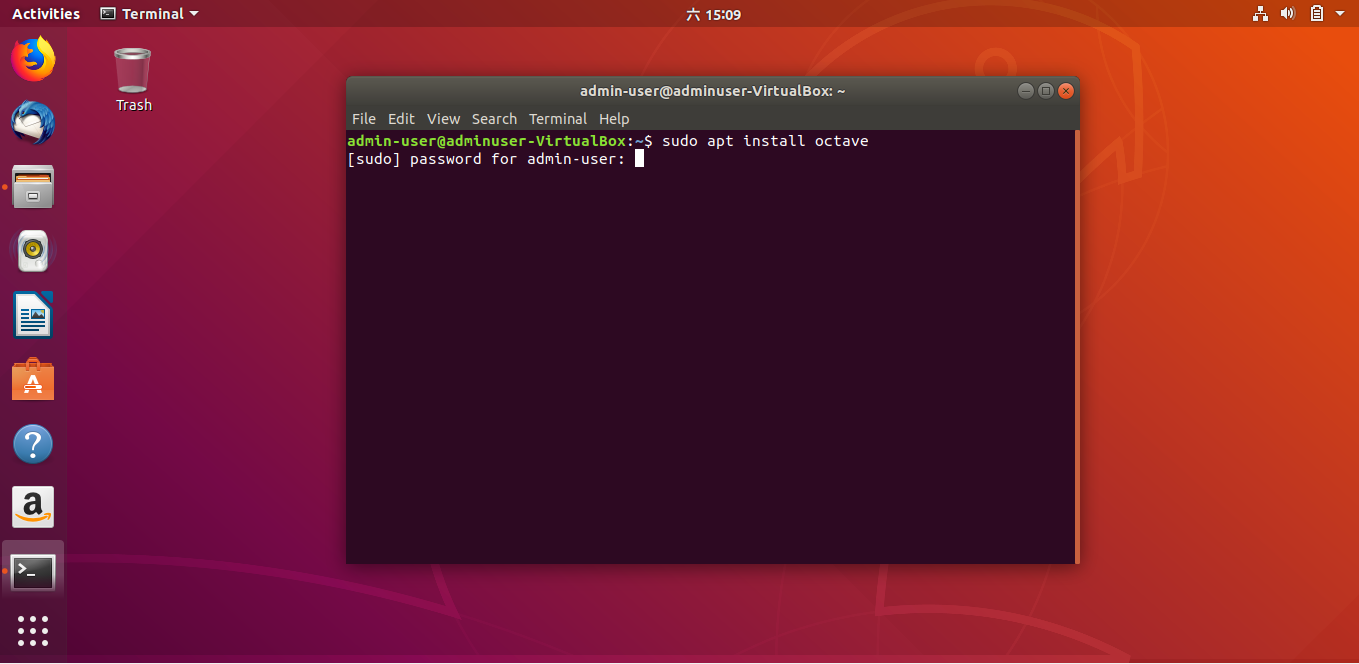
\includegraphics[width=\linewidth]{ubuntu2.png}

敲回车,然后让你输入刚才装系统时你给自己账户设置的密码(Linux中密码很重要,很多事情都要输入密码,瞎设密码导致忘了的话就凉了)。然后你会发现好像程序和卡死了一样,输入密码也不出现“***”什么的。这其实是Linux保护用户密码的机制,为了防止密码被偷窥所以输入密码时连位数都不回显。

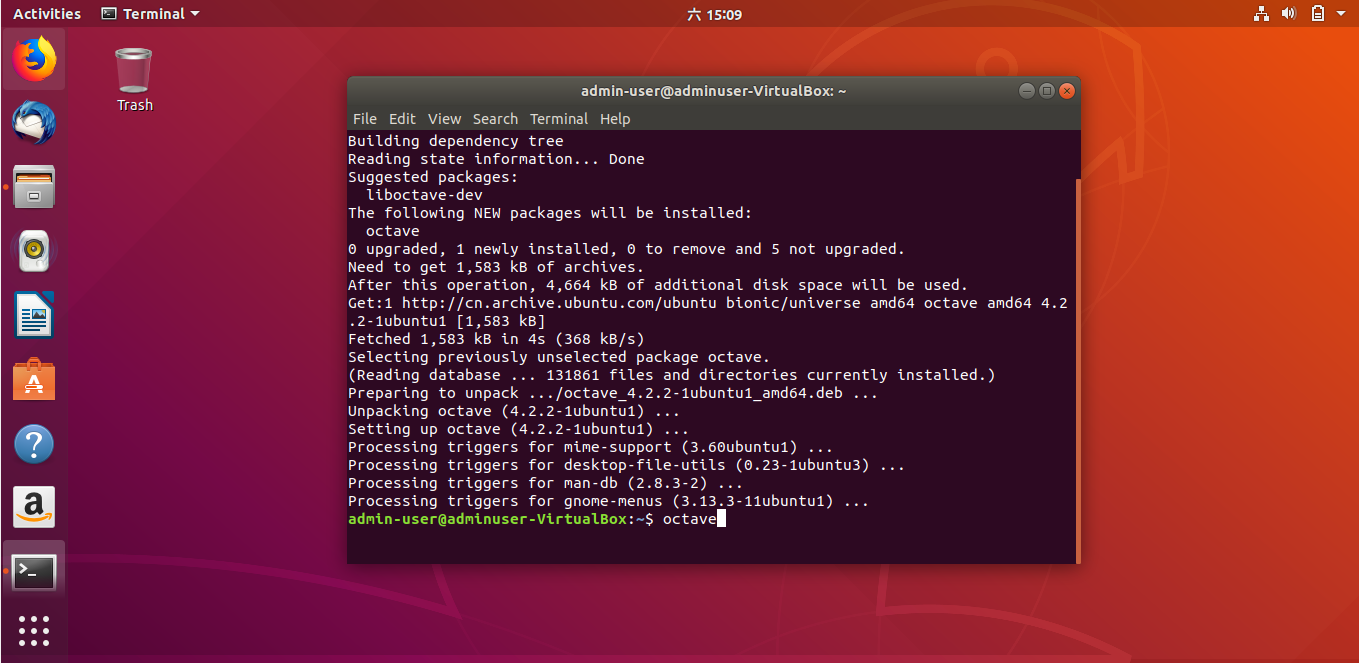
\includegraphics[width=\linewidth]{ubuntu3.png}

然后屏幕上就会打印出各种安装状态,也可能会向你确认是否安装。然后一切都安装好后,再在里面输入\texttt{octave},或者再去那个“所有应用程序”的界面找Octave的图标。

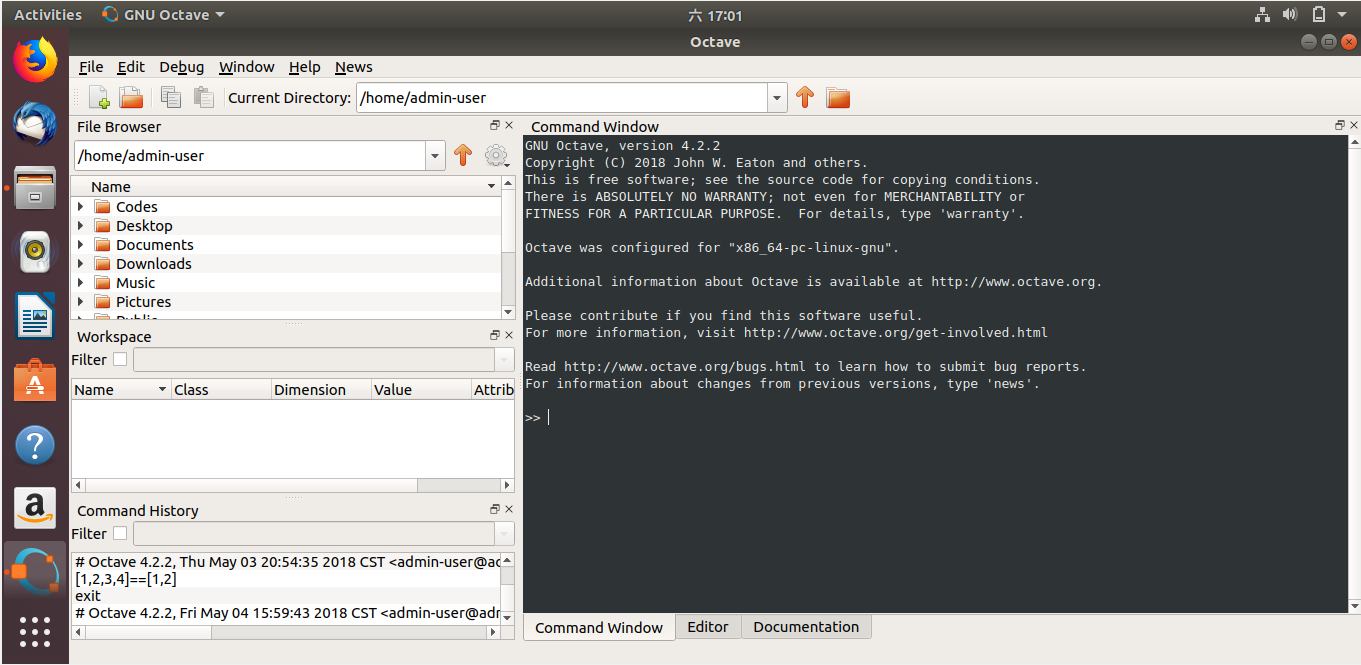
\includegraphics[width=\linewidth]{octave_ubuntu.png}

然后就可以和Windows和Mac上一样愉快的玩耍了。

\begin{center}
    [本期完]
\end{center}


\begin{center}

\includegraphics{by.png}

\small{

对本文章的使用,请遵循知识共享 4.0 (CC-BY 4.0)许可证。

本文章隶属于“Learn More CS, UNNC!”知识共享项目。

原项目地址:https://github.com/E-train-Liu/LearnMoreCS-UNNC

原项目 $ L ^{A} T _{E} X  $ 源代码使用遵循Apache 2.0协议,

原代码项目地址:https://github.com/E-train-Liu/LearnMoreCS-UNNC\_sourcecodes

© Copyright [2018] E-train-Liu
}
\end{center}


\end{spacing}
\end{document}

